
\documentclass[journal]{IEEEtran}
\usepackage{cite}
\usepackage{amsmath,amssymb,amsfonts}
\usepackage{graphicx}
\usepackage{booktabs}
\usepackage{array}
\usepackage[spanish,es-tabla]{babel}
\usepackage[utf8]{inputenc}
\usepackage[T1]{fontenc}
\usepackage{url}

\begin{document}

\title{Detección de URLs de \textit{phishing} mediante aprendizaje supervisado sobre el conjunto de datos PhiUSIIL}

\author{Julián Andrés Agudelo Echeverri, Mateo Reyes Uribe y Cristian Lizarazo Camaño%
\thanks{Los autores pertenecen a la Facultad de Ingeniería, Universidad de Antioquia. Proyecto del
curso Introducción al Machine Learning. Correos: julian.agudelo1@gmail.com,
mateo.reyesu@udea.edu.co, cristian.lizarazoc@udea.edu.co.}}

\markboth{Introducción al Machine Learning, Universidad de Antioquia}%
{Agudelo, Reyes y Lizarazo: Detección de URLs de \textit{phishing} sobre PhiUSIIL}

\maketitle

\begin{abstract}
El \textit{phishing} basado en URLs es una de las amenazas de ingeniería social más
extendidas y las listas negras tradicionales no alcanzan a cubrir los sitios creados
cada día. Este trabajo aborda la detección automática de URLs de \textit{phishing} como
un problema de clasificación binaria supervisada, empleando el conjunto de datos público
PhiUSIIL (235.795 URLs y 54 características léxicas, derivadas y del código HTML). El análisis
exploratorio revela que varias variables separan las clases casi de forma determinista por cómo
se construyó el conjunto, por lo que el escenario principal usa solo 19 variables calculadas a
partir de la URL. Se comparan cinco modelos con validación cruzada agrupada por dominio y MCC como
métrica principal. MLP y SVM con \textit{kernel} RBF obtienen MCC de prueba de 0,996, mientras que
la regresión logística alcanza 0,909; con todas las variables, incluso la regresión logística
llega a 0,9998. La selección de variables reduce el espacio a 9 variables sin pérdida apreciable,
PCA necesita 14 componentes para conservar el desempeño y UMAP pierde más de 0,15 en MCC. Los
resultados muestran que las cifras cercanas al 100\,\% sobre PhiUSIIL dependen en buena parte de la
construcción del conjunto.
\end{abstract}

\begin{IEEEkeywords}
phishing, detección de URLs, clasificación, aprendizaje supervisado, seguridad informática.
\end{IEEEkeywords}

%=============================================================================
\section{Introducción}
%=============================================================================
El \textit{phishing} es un ataque en el que un sitio web fraudulento suplanta a una entidad
legítima para robar credenciales o información financiera de los usuarios. Las defensas
basadas en listas negras son reactivas: solo bloquean URLs ya reportadas, por lo que fallan
ante los sitios nuevos, que tienen además un tiempo de vida muy corto. Esto motiva el uso de
\textit{machine learning} para aprender, a partir de características de la URL y de la página,
patrones que permitan clasificar un sitio como legítimo o fraudulento de forma automática y
anticipada.

El objetivo de este proyecto es construir y validar un modelo de aprendizaje supervisado que
clasifique una URL como legítima o de \textit{phishing} a partir del conjunto de datos
PhiUSIIL \cite{prasad2024}. El documento presenta la descripción del problema con su análisis
exploratorio (Sección~\ref{sec:problema}), la revisión del estado del arte
(Sección~\ref{sec:estado}), el entrenamiento y la evaluación de los modelos
(Sección~\ref{sec:modelos}), la reducción de dimensión (Sección~\ref{sec:reduccion}) y las
conclusiones (Sección~\ref{sec:conclusiones}). El código que reproduce los resultados
está disponible en el repositorio del proyecto\footnote{\url{https://github.com/mateor32/proyecto-modelos2-phishing}}.

%=============================================================================
\section{Descripción del problema}
\label{sec:problema}
%=============================================================================

\subsection{Contexto y utilidad de la solución}
Se busca decidir, de forma automática, si una URL corresponde a un sitio legítimo o a uno de
\textit{phishing}. Una solución basada en ML es útil porque generaliza a URLs no vistas (a
diferencia de las listas negras), puede integrarse en navegadores, clientes de correo o
\textit{gateways} de red, y opera en tiempo casi real. El reto es mantener una alta tasa de
detección con una baja tasa de falsos positivos, ya que bloquear sitios legítimos degrada la
experiencia del usuario.

\subsection{Descripción del conjunto de datos}
El conjunto de datos PhiUSIIL \cite{prasad2024}, disponible en el UCI Machine Learning
Repository, contiene \textbf{235.795 muestras} y \textbf{54 características} más la variable
objetivo. Cada muestra representa una URL y su página web asociada. Las clases se distribuyen en
\textbf{134.850 URLs legítimas} (\texttt{label}=1, 57,2\,\%) y \textbf{100.945 URLs de
\textit{phishing}} (\texttt{label}=0, 42,8\,\%), por lo que el problema está
\emph{moderadamente balanceado} (Fig.~\ref{fig:balance}). Las características se agrupan en tres
familias:
\begin{itemize}
  \item \textbf{Léxicas/estructurales de la URL:} \texttt{URLLength}, \texttt{DomainLength},
        \texttt{NoOfSubDomain}, \texttt{NoOfDegitsInURL}, \texttt{SpacialCharRatioInURL},
        \texttt{IsDomainIP}, entre otras.
  \item \textbf{Derivadas:} \texttt{URLSimilarityIndex}, \texttt{CharContinuationRate},
        \texttt{TLDLegitimateProb}, \texttt{URLCharProb}, calculadas por los autores a partir
        de otras variables o de una lista externa de sitios.
  \item \textbf{Del código HTML:} \texttt{LineOfCode}, \texttt{HasTitle}, \texttt{HasFavicon},
        \texttt{IsResponsive}, \texttt{HasPasswordField}, \texttt{NoOfJS},
        \texttt{HasCopyrightInfo}, \texttt{HasSocialNet}, etc.
\end{itemize}
Además hay cuatro variables de texto: \texttt{URL}, \texttt{Domain}, \texttt{TLD} y
\texttt{Title}. En cuanto a tipos, 50 variables son numéricas (de las cuales 19 son binarias
0/1) y 4 son de texto/categóricas.

\textbf{Datos faltantes y repetidos.} El conjunto \emph{no presenta valores faltantes} en
ninguna columna, por lo que no se requiere una estrategia de imputación. Tampoco existen filas
completamente duplicadas, pero 425 filas repiten una URL ya presente (sin conflicto de etiqueta)
y 5.526 dominios tienen más de una fila, con 21.235 muestras en total (p.\,ej.
\texttt{ipfs.io}, con 1.197); 54 de esos dominios tienen URLs de ambas clases. Por ello, antes de
particionar se eliminan las URLs repetidas y la partición se hace por dominio, de modo que un
mismo dominio no aparezca a la vez en entrenamiento y prueba.

\textbf{Codificación de variables.} Las variables de texto \texttt{URL}, \texttt{Domain} y
\texttt{Title} tienen una cardinalidad cercana al número de muestras (p.\,ej. 235.370 URLs
únicas), por lo que son prácticamente identificadores y no se codifican con \textit{one-hot};
se descartan como variables directas o se reservan para una posible extracción de
características de texto. La variable \texttt{TLD} tiene 695 categorías sin orden; dado que un
\textit{one-hot} generaría cientos de columnas dispersas, no se codifica directamente; la variable
numérica \texttt{TLDLegitimateProb}, que ya la resume como una probabilidad, se usa solo en el
escenario Completo de la Sección~\ref{sec:modelos}. Las variables numéricas tienen escalas muy distintas y colas largas (p.\,ej.
\texttt{LineOfCode} con máximo de 442.666), por lo que a los modelos sensibles a la escala se les aplica
$\log(1+x)$ y \textbf{estandarización} (\texttt{StandardScaler}), ajustadas solo sobre el
conjunto de entrenamiento.

\begin{figure}[t]
  \centering
  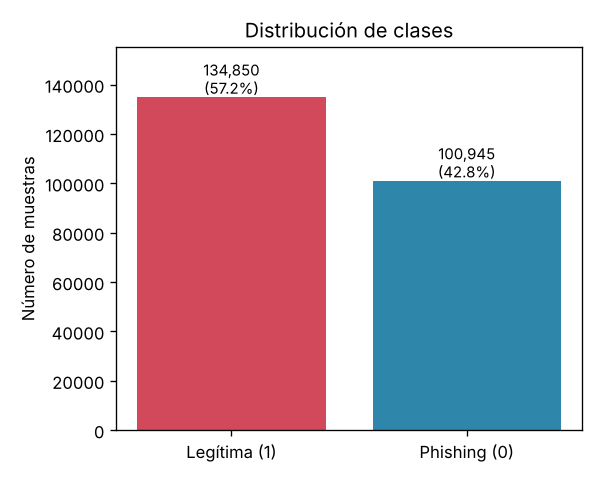
\includegraphics[width=0.85\columnwidth]{figures/01_class_balance.png}
  \caption{Distribución de clases del conjunto PhiUSIIL (57,2\,\% legítimas, 42,8\,\% phishing).}
  \label{fig:balance}
\end{figure}

\subsection{Análisis exploratorio}
El análisis de correlación muestra que varias características del código HTML y derivadas
separan bien las clases: \texttt{URLSimilarityIndex} ($\rho\approx0{,}86$),
\texttt{HasSocialNet} ($0{,}78$), \texttt{HasCopyrightInfo} ($0{,}74$) y \texttt{IsHTTPS}
($0{,}61$). Se identificó una posible \textbf{fuga de información}: todas las URLs legítimas usan
HTTPS y toda URL sin HTTPS es de \textit{phishing}, aunque 49.689 URLs de \textit{phishing}
(49,2\,\%) también usan HTTPS. Además, todas las legítimas tienen
\texttt{URLSimilarityIndex}=100, frente al 0,78\,\% del \textit{phishing}, algo esperable porque
ese índice compara cada URL con la lista Open PageRank de la que se obtuvieron las legítimas
\cite{prasad2024}; todas empiezan por
\texttt{www} (41,4\,\% del \textit{phishing}) y ninguna tiene ruta ni parámetros (28,2\,\% del
\textit{phishing} sí los tiene). Estos patrones sugieren que parte de la separación proviene de
la construcción del conjunto y no de una sola variable, lo que podría inflar el desempeño. Por
ello, la Sección~\ref{sec:modelos} evalúa el efecto de estas variables y de los distintos grupos
de características para valorar si el modelo generaliza. El detalle del EDA (dimensiones, tipos, duplicados, cardinalidad, distribuciones y correlaciones)
se encuentra en el notebook del repositorio, que comparte las mismas secciones de este informe.

\subsection{Paradigma de aprendizaje}
El problema se enmarca en el \textbf{aprendizaje supervisado}, ya que se dispone de un conjunto
de pares etiquetados $\mathcal{D}=\{(\mathbf{x}_i,y_i)\}_{i=1}^{N}$ con $y_i\in\{0,1\}$. Como la
variable de salida es categórica (legítima / phishing), se trata de un problema de
\textbf{clasificación binaria}. Este paradigma es el apropiado porque el objetivo es predecir
una etiqueta conocida a partir de ejemplos previos, y no descubrir estructura latente (lo que
correspondería a aprendizaje no supervisado). Dado el balance moderado de clases y la repetición
de dominios, se usa una partición \textbf{estratificada y agrupada por dominio} y, además de la exactitud, se
reportan métricas robustas al desbalance como F1, MCC y el área bajo la curva ROC (AUC).

%=============================================================================
\section{Estado del arte}
\label{sec:estado}
%=============================================================================
La Tabla~\ref{tab:sota} resume trabajos que abordan la detección de \textit{phishing} por URL
usando el conjunto de datos PhiUSIIL. El trabajo original \cite{prasad2024} introduce el
conjunto de datos y un marco de detección basado en un \emph{índice de similitud} de la URL y
\emph{aprendizaje incremental}, que permite actualizar el modelo ante URLs nuevas.
Posteriormente, \cite{gobinath2026} propone una red neuronal profunda con mecanismo de atención
\textit{multi-head} (ADUIN) orientada a la detección de ataques de día cero, sobre un corpus que
combina PhiUSIIL con datos de Kaggle y Mendeley, mientras que \cite{bao2026} compara algoritmos
clásicos (Random Forest, SVM, Naïve Bayes y una red MLP) y reporta exactitudes superiores al
99\,\% sobre PhiUSIIL. Finalmente, \cite{yulianti2026} estudia métodos de selección de
características con 20 variables de la URL, pues excluye las del contenido de la página y trata
\texttt{URLSimilarityIndex} y \texttt{TLDLegitimateProb} como fuga de información; con LASSO
($k=5$ variables) obtiene un F1 equivalente al de las 20 variables.

Una métrica ajena a la sesión de métricas del curso que aparece en \cite{bao2026} es la
\textbf{pérdida logarítmica}, que penaliza las probabilidades mal calibradas:
\begin{equation}
\mathcal{L} = -\frac{1}{N}\sum_{i=1}^{N}\left[y_i\log p_i + (1-y_i)\log(1-p_i)\right],
\end{equation}
donde $p_i$ es la probabilidad estimada de la clase positiva. La detección de día cero de
\cite{gobinath2026} es la proporción de URLs de \textit{phishing} no vistas que se detectan. Las
demás métricas reportadas (exactitud, precisión, \textit{recall}, F1, MCC, FPR y AUC) se estudiaron
en el curso.

% ---- Tabla comparativa (máx. 1 página para toda la sección) ----
\begin{table*}[t]
\centering
\caption{Trabajos que emplean el conjunto de datos PhiUSIIL.}
\label{tab:sota}
\small
\begin{tabular}{p{2.6cm} p{1.6cm} p{3.0cm} p{2.6cm} p{2.4cm} p{2.6cm}}
\toprule
\textbf{Trabajo} & \textbf{Paradigma} & \textbf{Técnica(s)} & \textbf{Validación} & \textbf{Métricas} & \textbf{Resultados} \\
\midrule
Prasad \& Chandra, 2024 \cite{prasad2024} \newline \textit{Computers \& Security} (Elsevier) &
Supervisado (clasif.) &
Índice de similitud de URL + aprendizaje incremental (BernoulliNB, Passive-Aggressive, SGD) &
Flujo incremental sobre todo el conjunto; pre-entrenamiento con divisiones de 10:90 a 90:10 &
Exactitud, precisión, sensibilidad, F1, MCC &
99,24\,\% (incremental); 99,79\,\% (pre-entrenamiento, 90:10) \\
\addlinespace
Gobinath \& Manikandan, 2026 \cite{gobinath2026} \newline \textit{Scientific Reports} (Nature) &
Supervisado (clasif.) &
Red neuronal profunda con atención \textit{multi-head} (ADUIN); \textit{baselines}: SVM, RF, LR. Datos: PhiUSIIL, Kaggle y Mendeley &
División 70/15/15 + 10 repeticiones estratificadas (t-test, McNemar) &
Exactitud, precisión, recall, F1, FPR, detección día-cero &
95\,\% exactitud; 93\,\% precisión; 92\,\% detección día-cero; FPR 3,5\,\% \\
\addlinespace
Bao \textit{et al.}, 2026 \cite{bao2026} \newline \textit{Computers, Materials \& Continua} &
Supervisado (clasif.) &
Random Forest, SVM, Naïve Bayes, red MLP &
Hold-out estratificado 80/20 (+ k-fold) &
Exactitud, precisión, recall, F1, ROC-AUC, log-loss &
Exactitud: RF 99,99\,\%; MLP 99,98\,\%; SVM 99,97\,\%; NB 99,94\,\% \\
\addlinespace
Yulianti \& Forenziana, 2026 \cite{yulianti2026} \newline \textit{Formosa J. of Comp. and Inf. Science} &
Supervisado (clasif.) &
Selección de características (filtro, \textit{wrapper}, embebido/LASSO) con 20 variables de URL &
Hold-out estratificado 80/20 + 5-fold estratificado &
Exactitud, precisión, recall, F1, ROC-AUC &
LASSO ($k{=}5$): F1 0,9975 vs. 0,9965 con 20 variables \\
\bottomrule
\end{tabular}
\end{table*}

\textbf{Observación.} Los desempeños reportados sobre PhiUSIIL son muy altos ($>99\,\%$ en varios
casos), lo que es coherente con la fuerte asociación de algunas características con la etiqueta
observada en el EDA. Esto, junto con la exclusión de variables hecha en \cite{yulianti2026},
refuerza la necesidad de un protocolo de validación cuidadoso, que se describe en la
Sección~\ref{sec:modelos}.

%=============================================================================
\section{Entrenamiento y evaluación de los modelos}
\label{sec:modelos}
%=============================================================================
\subsection{Configuración experimental}

\textbf{Escenarios.} Tras eliminar las URLs repetidas quedan 235.370 muestras, con 42,7\,\% de
\textit{phishing}, que se toma como clase positiva. Se definen dos escenarios. El escenario
principal, \textbf{Solo URL}, usa 19 variables calculadas a partir de la URL y excluye las 28 del
código HTML, además de \texttt{URLSimilarityIndex}, \texttt{IsHTTPS} y \texttt{TLDLegitimateProb},
por la fuga identificada en la Sección~\ref{sec:problema}. Se conserva \texttt{URLCharProb}, que es
una tabla general de frecuencias aplicable a cualquier URL, aunque se construyó con la misma lista
de sitios legítimos. El escenario \textbf{Completo} usa las 50 variables numéricas y sirve de
referencia para medir el efecto de las variables retiradas.

\textbf{Metodología de validación.} La prueba reserva el 20\,\% de las muestras (47.074: 20.104 de
\textit{phishing} y 26.970 legítimas) y las 188.296 restantes se usan para entrenar. La partición es
estratificada y agrupada por dominio, por lo que ambos conjuntos no comparten ningún dominio. Los
hiperparámetros se eligen con validación cruzada estratificada y agrupada de 5 pliegues
(\texttt{StratifiedGroupKFold}), de modo que la prueba no interviene en la elección de
hiperparámetros ni de modelos. La malla completa se ejecuta en el escenario Solo URL; el escenario Completo reutiliza
los mejores hiperparámetros encontrados, para que la comparación refleje el cambio de variables.

\textbf{Preprocesamiento.} Las variables tienen colas largas, de modo que se aplica $\log(1+x)$ y
estandarización dentro de un \texttt{Pipeline}, ajustado solo con los datos de entrenamiento de
cada pliegue. Random Forest no lo requiere porque los árboles no dependen de la escala. No se usa
remuestreo, dado que el desbalance es moderado. Por su costo computacional, SVM se entrena con un
subconjunto de 31.383 muestras tomado por dominios; su evaluación de prueba sí usa las 47.074
muestras.

\textbf{Métricas.} La métrica de selección es el coeficiente de correlación de Matthews
\begin{equation}
\mathrm{MCC}=\frac{TP\cdot TN-FP\cdot FN}{\sqrt{(TP+FP)(TP+FN)(TN+FP)(TN+FN)}},
\end{equation}
porque tiene en cuenta las cuatro casillas de la matriz de confusión y no se ve favorecido por la
clase mayoritaria. Además se reportan exactitud, F1, AUC y la tasa de falsos positivos (FPR), esta
última porque un falso positivo bloquea un sitio legítimo. Para entrenamiento y validación los
intervalos son la media $\pm$ 2 desviaciones estándar entre pliegues. La prueba es una sola
evaluación, por lo que su intervalo remuestrea 10.000 veces su matriz de confusión; este
procedimiento supone URLs independientes y puede quedar algo estrecho.

\textbf{Modelos y mallas.} La Tabla~\ref{tab:mallas} presenta los cinco modelos y las
configuraciones evaluadas. La red MLP usa lotes de 512 muestras, un máximo de 100 épocas y parada
temprana con una separación interna aleatoria del 10\,\%, que no agrupa por dominio y solo decide
cuándo detener el entrenamiento.

\begin{table*}[t]
\centering
\caption{Modelos, mallas de hiperparámetros y configuración elegida por MCC de validación.}
\label{tab:mallas}
\small
\begin{tabular}{p{2.7cm} p{2.2cm} p{6.3cm} c p{3.5cm}}
\toprule
\textbf{Modelo} & \textbf{Tipo} & \textbf{Malla} & \textbf{Config.} & \textbf{Elegida} \\
\midrule
Regresión logística & Paramétrico &
$C\in\{10^{-3},\dots,10^{2}\}$; penalización L1 o L2 & 12 & $C=100$, L2 \\
KNN & No paramétrico &
$k\in\{1,3,5,11,21,51\}$; pesos uniformes o por distancia & 12 & $k=1$, uniformes \\
Random Forest & Ensamble de árboles &
Árboles $\in\{50,100,200\}$; profundidad $\in\{10,20,\text{sin límite}\}$ & 9 &
200 árboles, profundidad 20 \\
MLP & Red neuronal &
Capas ocultas (32), (64, 32), (128, 64), (128, 64, 32); $\alpha\in\{10^{-4},10^{-2}\}$ & 8 &
(128, 64, 32), $\alpha=10^{-4}$ \\
SVM & Vectores de soporte &
RBF: $C\in\{0{,}1;1;10;100\}$, $\gamma\in\{0{,}01;0{,}1;1;\texttt{scale}\}$.
Lineal: $C\in\{0{,}1;1;10\}$ & 19 & RBF, $C=100$, $\gamma=\texttt{scale}$ \\
\bottomrule
\end{tabular}
\end{table*}

\subsection{Resultados del entrenamiento}

\textbf{Escenario Solo URL.} La Tabla~\ref{tab:solourl} muestra los resultados. Los modelos lineales
se quedan cerca de MCC 0,91: regresión logística alcanza 0,9091 y la mejor SVM lineal, 0,9152. Los
modelos no lineales superan 0,96, lo que indica que la frontera entre clases con estas variables
no es lineal. Los dos mejores por MCC de validación son \textbf{MLP} (0,9956 $\pm$ 0,0014) y
\textbf{SVM} (0,9949 $\pm$ 0,0041), que pasan a la Sección~\ref{sec:reduccion}. Sus intervalos se solapan, de
modo que estos resultados no permiten afirmar que uno sea superior, y SVM usó menos datos.

\begin{table*}[t]
\centering
\caption{Resultados del escenario Solo URL (media $\pm$ 2 desviaciones estándar). Las columnas de
exactitud a FPR corresponden a validación. El entrenamiento de KNN no se evaluó por pliegue: con
$k=1$ vale 1 por construcción. Entrenamiento y validación de SVM usan el subconjunto de 31.383
muestras.}
\label{tab:solourl}
\resizebox{\textwidth}{!}{%
\begin{tabular}{lccccccc}
\toprule
\textbf{Modelo} & \textbf{MCC entren.} & \textbf{MCC valid.} & \textbf{MCC prueba} &
\textbf{Exactitud} & \textbf{F1} & \textbf{AUC} & \textbf{FPR} \\
\midrule
Regresión logística & 0,9093 $\pm$ 0,0014 & 0,9091 $\pm$ 0,0015 & 0,9090 $\pm$ 0,0038 &
0,9555 $\pm$ 0,0007 & 0,9468 $\pm$ 0,0010 & 0,9806 $\pm$ 0,0020 & 0,0237 $\pm$ 0,0026 \\
KNN & -- & 0,9653 $\pm$ 0,0026 & 0,9678 $\pm$ 0,0023 &
0,9830 $\pm$ 0,0013 & 0,9801 $\pm$ 0,0015 & 0,9823 $\pm$ 0,0012 & 0,0126 $\pm$ 0,0016 \\
Random Forest & 0,9975 $\pm$ 0,0003 & 0,9911 $\pm$ 0,0015 & 0,9928 $\pm$ 0,0011 &
0,9957 $\pm$ 0,0007 & 0,9949 $\pm$ 0,0009 & 0,9985 $\pm$ 0,0006 & 0,0028 $\pm$ 0,0005 \\
MLP & 0,9959 $\pm$ 0,0006 & 0,9956 $\pm$ 0,0014 & 0,9960 $\pm$ 0,0008 &
0,9978 $\pm$ 0,0007 & 0,9975 $\pm$ 0,0008 & 0,9986 $\pm$ 0,0005 & 0,0002 $\pm$ 0,0002 \\
SVM & 0,9957 $\pm$ 0,0010 & 0,9949 $\pm$ 0,0041 & 0,9961 $\pm$ 0,0008 &
0,9975 $\pm$ 0,0020 & 0,9971 $\pm$ 0,0023 & 0,9977 $\pm$ 0,0024 & 0,0003 $\pm$ 0,0005 \\
\bottomrule
\end{tabular}}
\end{table*}

En MLP y SVM, entrenamiento, validación y prueba prácticamente coinciden, por lo que no se observa
sobreajuste. Random Forest presenta una brecha pequeña entre entrenamiento y validación. La
Fig.~\ref{fig:matriz} muestra que los errores de MLP son sobre todo \textit{phishing} no detectado:
91 falsos negativos (0,45\,\% del \textit{phishing}) frente a 2 falsos positivos. SVM tiene un
balance similar, con 85 y 6.

\begin{figure}[t]
  \centering
  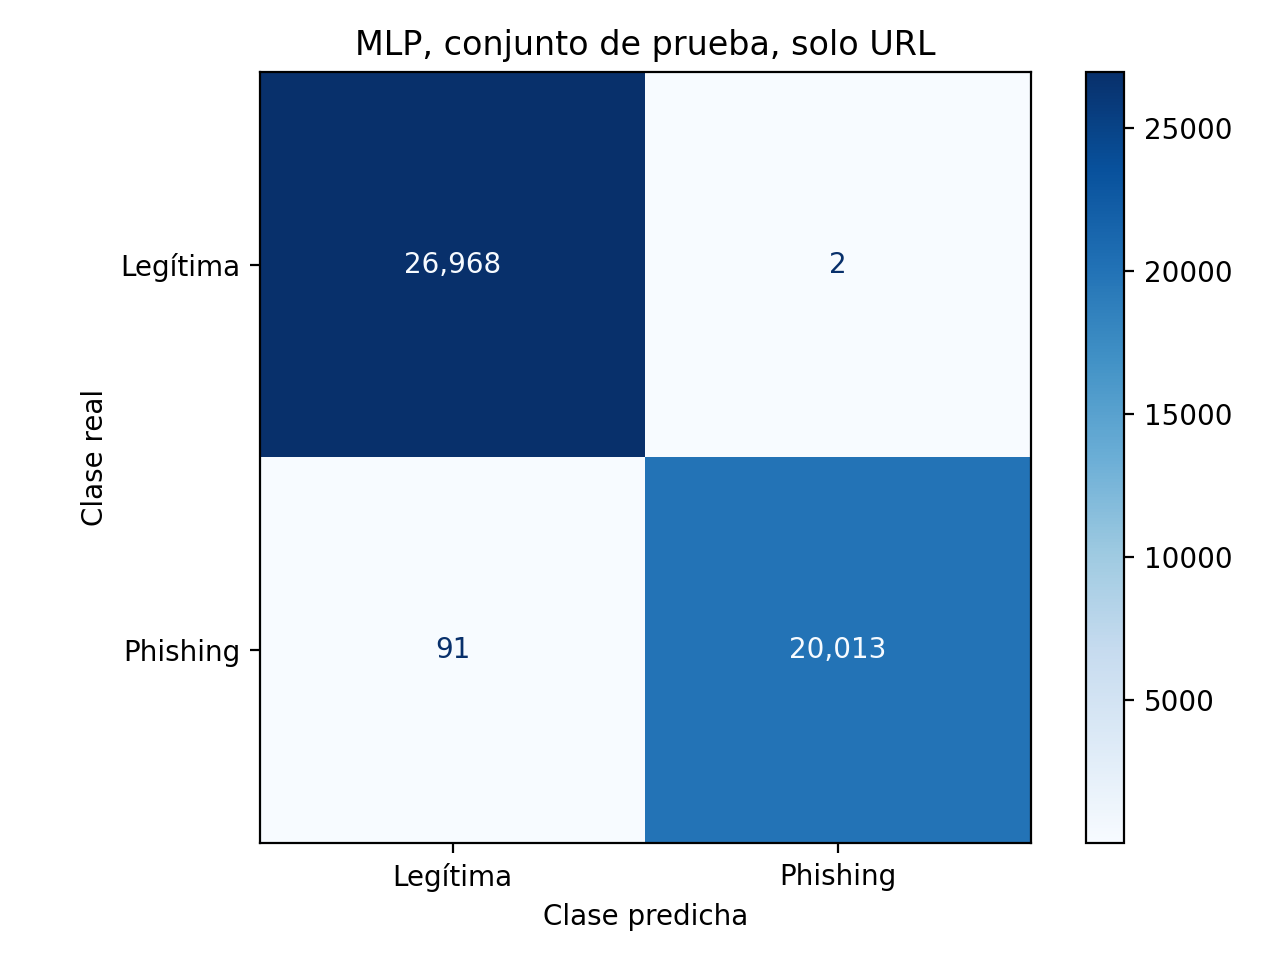
\includegraphics[width=0.8\columnwidth]{figures/matriz_confusion.png}
  \caption{Matriz de confusión de MLP en el conjunto de prueba, escenario Solo URL.}
  \label{fig:matriz}
\end{figure}

\textbf{Efecto de los hiperparámetros.} La Fig.~\ref{fig:hiper} muestra que regresión logística se
estabiliza desde $C=10$, con L1 y L2 equivalentes. En KNN el desempeño cae al aumentar $k$, de modo
que el mejor valor es el límite inferior posible; con él, una sola muestra decide la clase. En
Random Forest el salto ocurre entre las profundidades 10 y 20, sin límite baja levemente y el número
de árboles apenas influye. En SVM, $\gamma=1$ separa más entrenamiento y validación, lo que indica
sobreajuste. Varias configuraciones elegidas están en un extremo de la malla, pero las diferencias
con sus vecinas caen dentro de los intervalos o las curvas ya son planas; en la red MLP
(Fig.~\ref{fig:mlp}) ocurre lo mismo con la arquitectura, por lo que no se amplió la búsqueda.

\begin{figure*}[t]
  \centering
  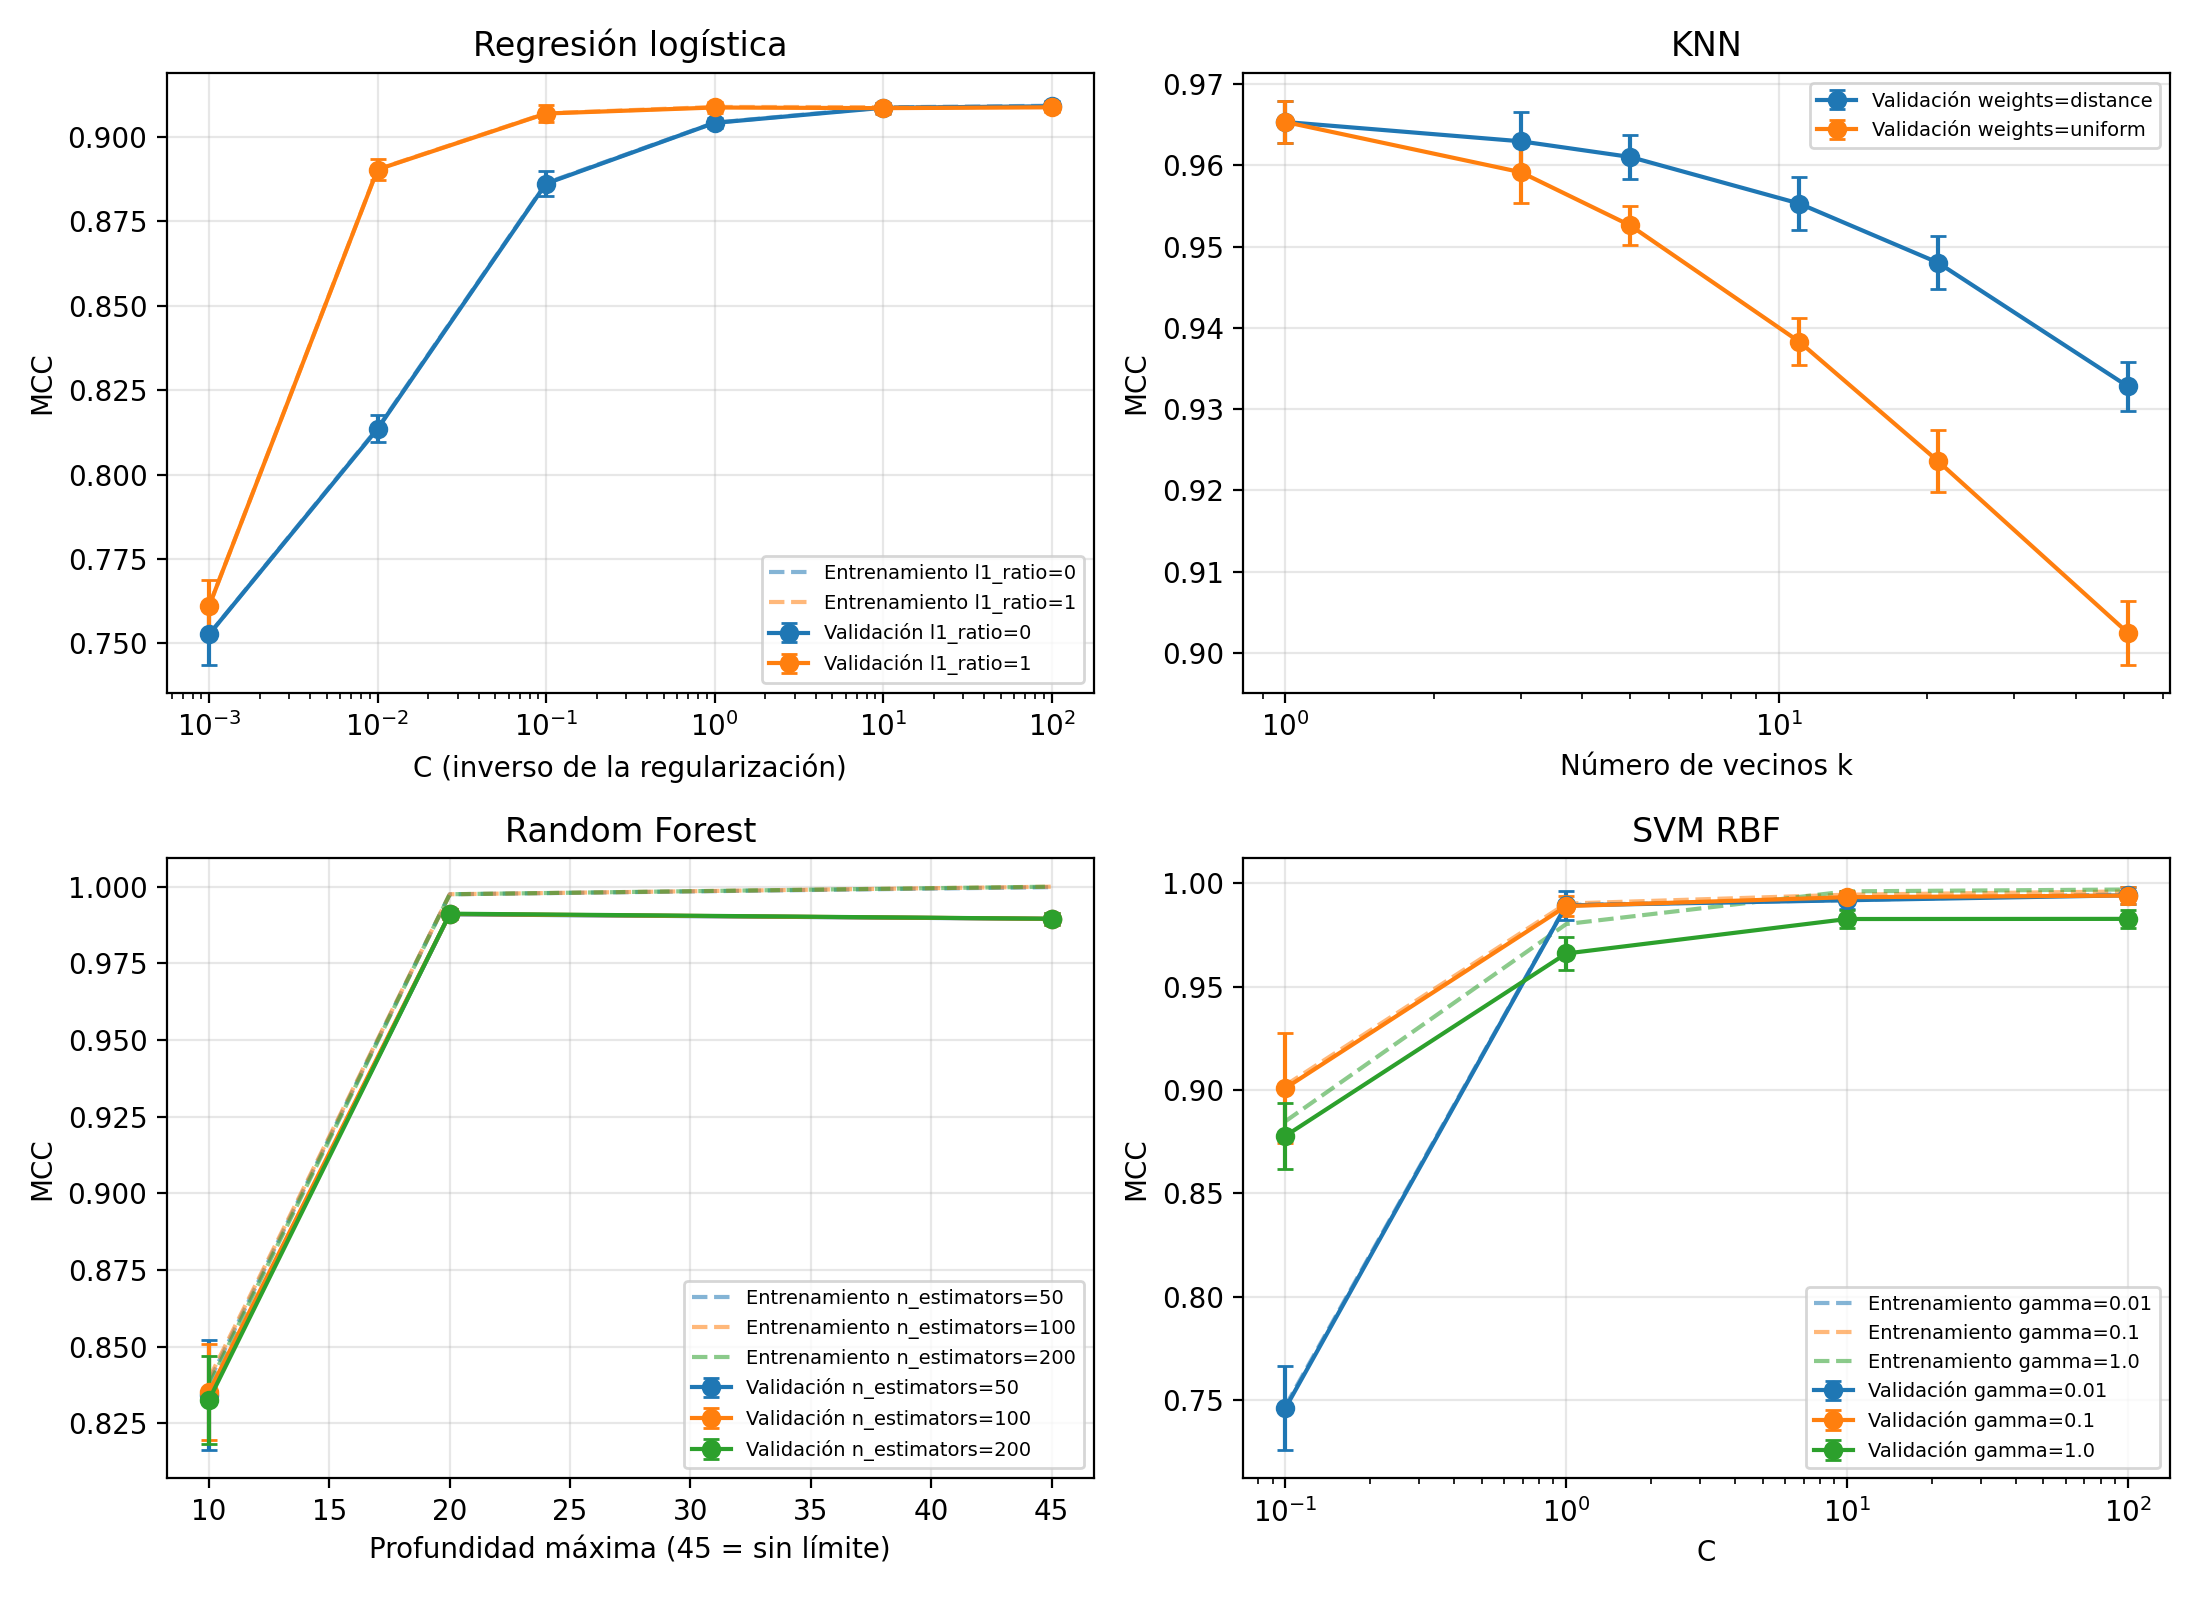
\includegraphics[width=0.85\textwidth]{figures/hiperparametros_modelos.png}
  \caption{MCC de entrenamiento (línea discontinua) y validación (línea continua, media $\pm$ 2
  desviaciones estándar) según los hiperparámetros. KNN no incluye entrenamiento y SVM usa el
  subconjunto de 31.383 muestras.}
  \label{fig:hiper}
\end{figure*}

\begin{figure}[t]
  \centering
  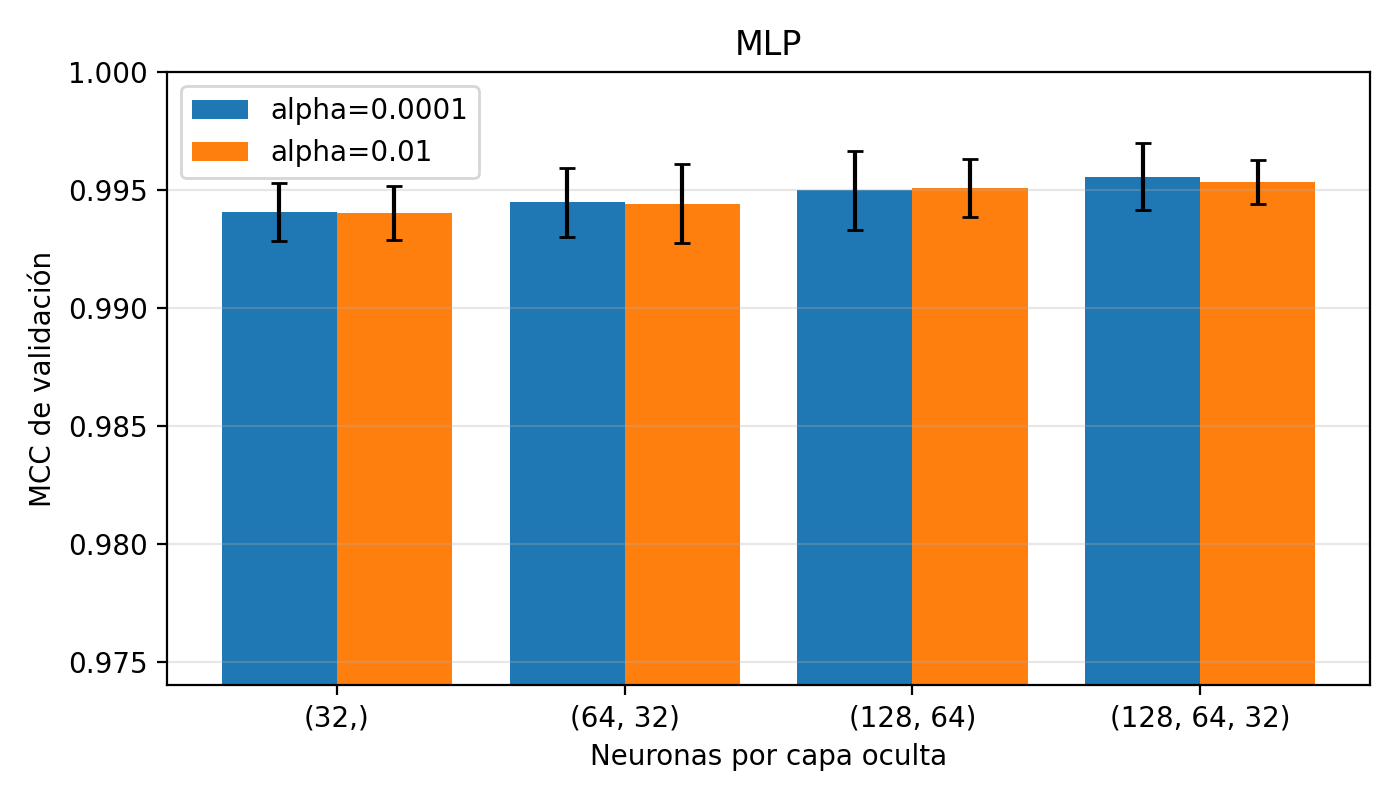
\includegraphics[width=\columnwidth]{figures/hiperparametros_mlp.png}
  \caption{MCC de validación (media $\pm$ 2 desviaciones estándar) de MLP según la arquitectura y
  la regularización $\alpha$.}
  \label{fig:mlp}
\end{figure}

\textbf{Escenario Completo.} La Tabla~\ref{tab:completo} y la Fig.~\ref{fig:escenarios} muestran que
todos los modelos llegan casi a la perfección al añadir las 31 variables retiradas, incluso
regresión logística, que pasa de 0,9091 a 0,9999. Esa mejora de un modelo lineal confirma que el
conjunto contiene señales casi deterministas, por lo que este escenario no mide la capacidad de
generalizar a sitios reales. Aun en Solo URL hay que interpretar el desempeño con cautela, porque
las URLs legítimas conservan la estructura descrita en la Sección~\ref{sec:problema}: todas
empiezan por \texttt{www} y ninguna tiene ruta.

\begin{table}[t]
\centering
\caption{Resultados del escenario Completo con los hiperparámetros elegidos en Solo URL. FP y FN se
cuentan en prueba.}
\label{tab:completo}
\begin{tabular}{lccrr}
\toprule
\textbf{Modelo} & \textbf{MCC valid.} & \textbf{MCC prueba} & \textbf{FP} & \textbf{FN} \\
\midrule
Reg. logística & 0,9999 $\pm$ 0,0001 & 0,9998 $\pm$ 0,0002 & 0 & 4 \\
KNN & 0,9985 $\pm$ 0,0004 & 0,9988 $\pm$ 0,0005 & 1 & 27 \\
Random Forest & 1,0000 $\pm$ 0,0001 & 1,0000 $\pm$ 0,0001 & 0 & 1 \\
MLP & 0,9998 $\pm$ 0,0001 & 0,9999 $\pm$ 0,0001 & 0 & 2 \\
SVM & 0,9999 $\pm$ 0,0005 & 0,9999 $\pm$ 0,0001 & 1 & 1 \\
\bottomrule
\end{tabular}
\end{table}

\begin{figure}[t]
  \centering
  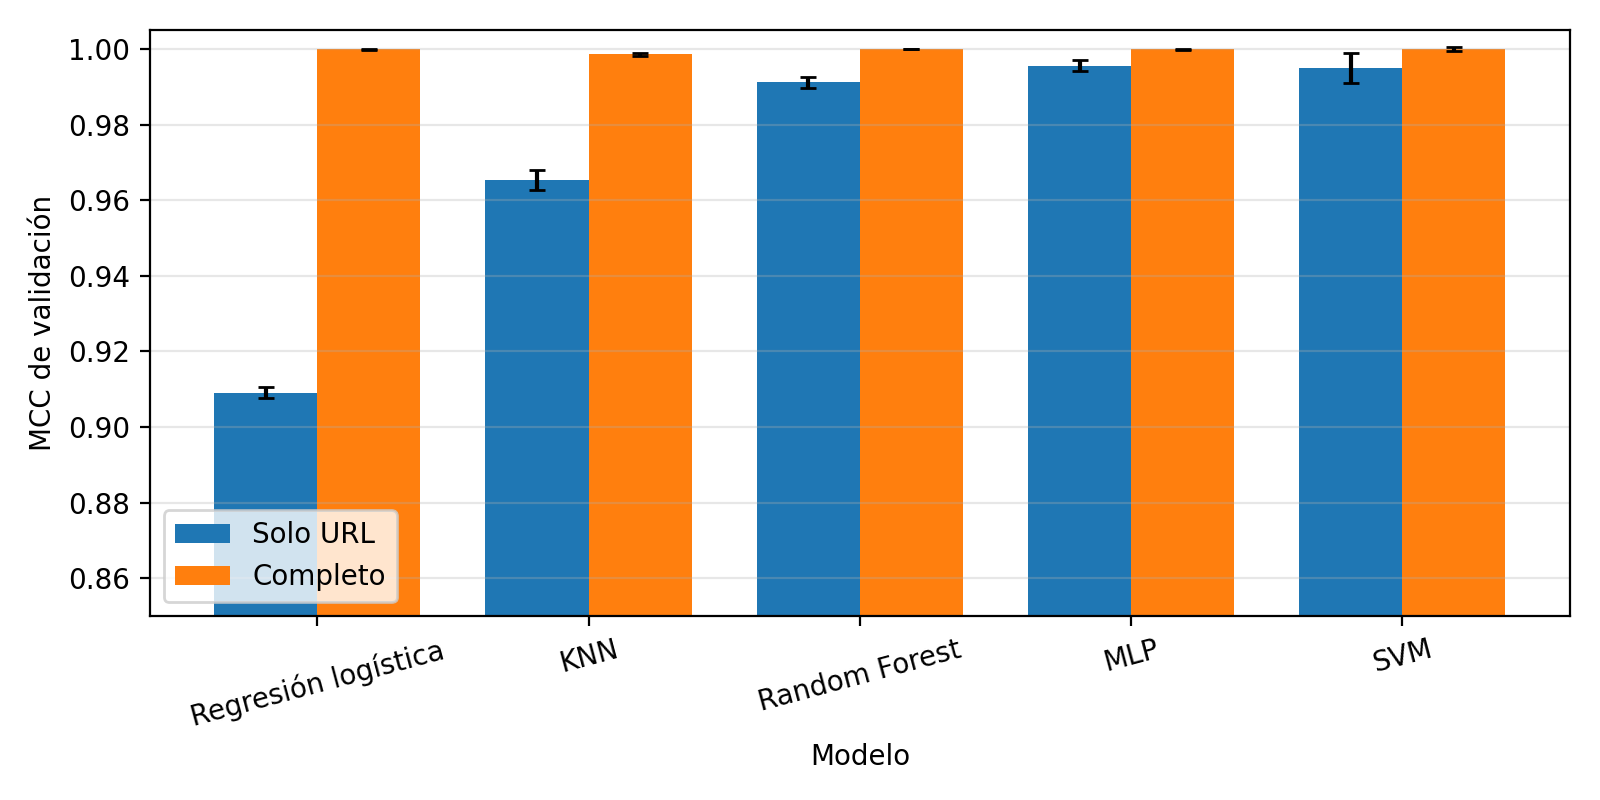
\includegraphics[width=\columnwidth]{figures/comparacion_escenarios.png}
  \caption{MCC de validación (media $\pm$ 2 desviaciones estándar) por modelo en los escenarios
  Solo URL y Completo.}
  \label{fig:escenarios}
\end{figure}

%=============================================================================
\section{Reducción de dimensión}
\label{sec:reduccion}
%=============================================================================
Esta sección trabaja sobre el escenario Solo URL con los dos mejores modelos de la
Sección~\ref{sec:modelos}, MLP y SVM. Se usan la misma partición de prueba y los mismos pliegues,
de modo que los resultados son comparables con la Tabla~\ref{tab:solourl}.

\subsection{Análisis individual y selección de variables}

Cada variable se evalúa con el conjunto de entrenamiento mediante tres índices. El índice de Fisher,
$J=(\mu_1-\mu_0)^2/(\sigma_1^2+\sigma_0^2)$, compara la separación de las medias de cada clase con
sus varianzas. El AUC univariado, tomado como $\max(\mathrm{AUC},1-\mathrm{AUC})$, mide qué tan bien
ordena la variable las clases por sí sola, donde 0,5 equivale al azar. La información mutua, estimada
con 40.000 muestras, capta también relaciones no monótonas. La redundancia se mide con la correlación
de Pearson entre variables. La Tabla~\ref{tab:variables} y la Fig.~\ref{fig:variables} muestran los
resultados.

\begin{table}[t]
\centering
\caption{Índices de discriminación de cada variable del escenario Solo URL, calculados en
entrenamiento y ordenados por AUC univariado. Las marcadas con $^{*}$ tienen AUC $<0{,}55$.}
\label{tab:variables}
\footnotesize
\begin{tabular}{lccc}
\toprule
\textbf{Variable} & \textbf{Fisher} & \textbf{AUC} & \textbf{Inf. mutua} \\
\midrule
NoOfOtherSpecialCharsInURL & 0,3650 & 0,8233 & 0,2357 \\
SpacialCharRatioInURL & 0,7626 & 0,8099 & 0,2113 \\
URLCharProb & 0,5316 & 0,7663 & 0,1295 \\
CharContinuationRate & 0,5514 & 0,7488 & 0,1612 \\
NoOfLettersInURL & 0,1428 & 0,7406 & 0,1501 \\
URLLength & 0,1280 & 0,7307 & 0,1634 \\
NoOfDegitsInURL & 0,1010 & 0,7266 & 0,1696 \\
DegitRatioInURL & 0,3990 & 0,7247 & 0,1650 \\
LetterRatioInURL & 0,2985 & 0,7134 & 0,3784 \\
DomainLength & 0,1683 & 0,6285 & 0,0847 \\
NoOfQMarkInURL$^{*}$ & 0,0552 & 0,5305 & 0,0239 \\
TLDLength$^{*}$ & 0,0145 & 0,5289 & 0,0140 \\
NoOfEqualsInURL$^{*}$ & 0,0194 & 0,5267 & 0,0203 \\
NoOfSubDomain$^{*}$ & 0,0004 & 0,5102 & 0,0673 \\
NoOfAmpersandInURL$^{*}$ & 0,0027 & 0,5043 & 0,0000 \\
IsDomainIP$^{*}$ & 0,0068 & 0,5034 & 0,0019 \\
ObfuscationRatio$^{*}$ & 0,0028 & 0,5023 & 0,0006 \\
HasObfuscation$^{*}$ & 0,0045 & 0,5023 & 0,0000 \\
NoOfObfuscatedChar$^{*}$ & 0,0005 & 0,5023 & 0,0000 \\
\bottomrule
\end{tabular}
\end{table}

\begin{figure*}[t]
  \centering
  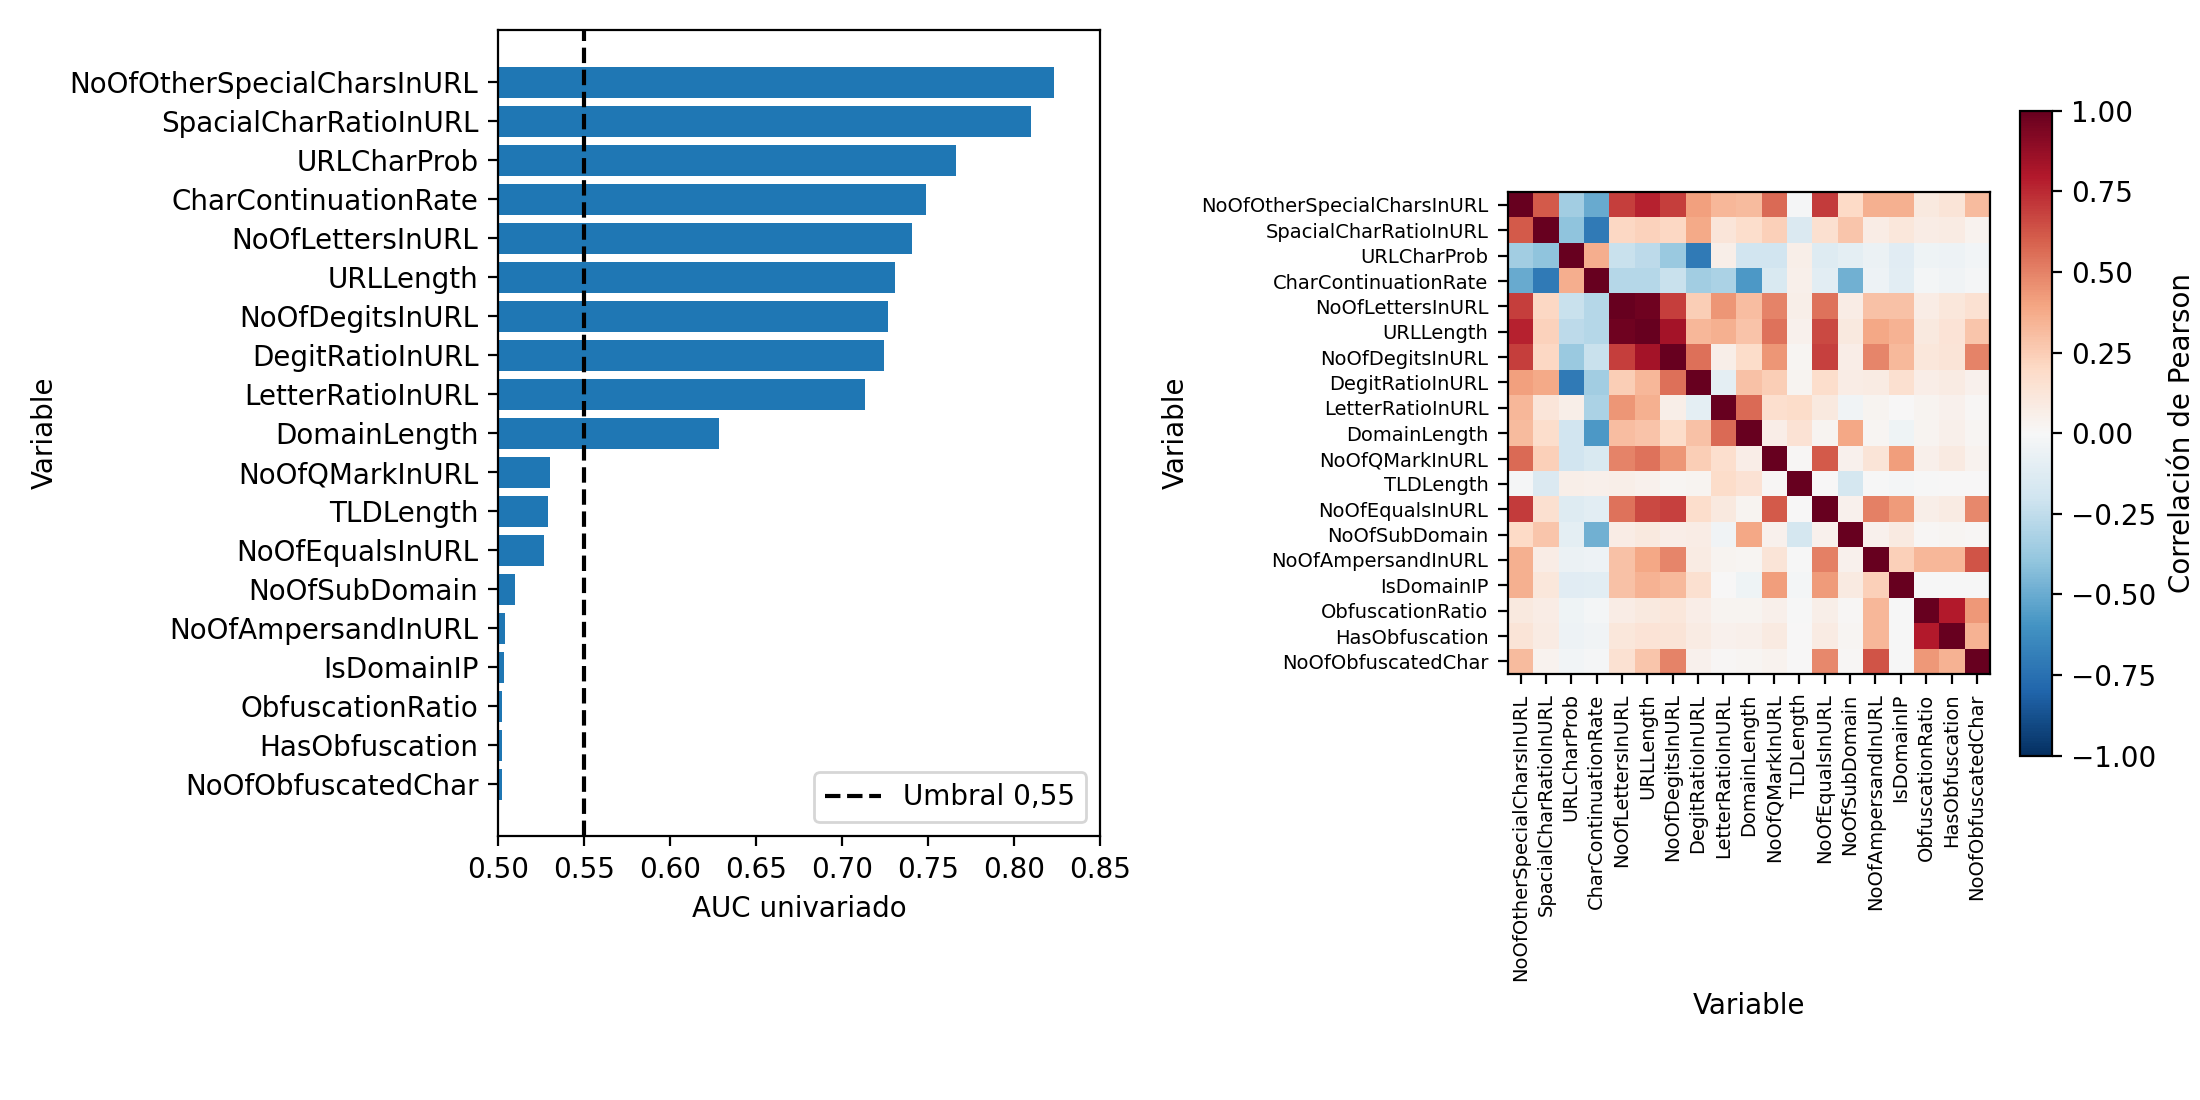
\includegraphics[width=0.85\textwidth]{figures/analisis_variables.png}
  \caption{Izquierda: AUC univariado de cada variable del escenario Solo URL, con el umbral de 0,55
  usado para marcarlas como débiles. Derecha: correlación de Pearson entre variables, en el mismo
  orden. Ambos se calculan con el conjunto de entrenamiento.}
  \label{fig:variables}
\end{figure*}

Las variables que cuentan caracteres especiales y la probabilidad de caracteres son las más
discriminantes, con AUC entre 0,77 y 0,82. En el otro extremo, nueve variables tienen AUC menor que
0,55. Las tres de ofuscación e \texttt{IsDomainIP} son distintas de cero en menos del 0,3\,\% de las
URLs, por lo que casi no aportan información. \texttt{NoOfSubDomain} es un caso particular: su AUC es 0,51, pero su
información mutua (0,067) es mayor que la de otras débiles, lo que sugiere una relación no monótona
con la clase. En cuanto a redundancia, el único par con correlación absoluta de al menos 0,95 es
\texttt{URLLength} y \texttt{NoOfLettersInURL} ($r=0{,}974$).

Una variable débil por sí sola puede aportar en combinación con otras, así que los índices solo
proponen candidatas a eliminar. Antes de evaluar se fijan tres criterios: quitar la variable de menor
AUC de cada par con $|r|\ge0{,}95$ (redundantes), quitar las de AUC $<0{,}55$ (débiles) y quitar solo
las débiles que además tienen información mutua $<0{,}01$. Cada conjunto se evalúa con los
hiperparámetros elegidos en la Sección~\ref{sec:modelos} y los mismos pliegues. Se elige el conjunto
más pequeño cuyo MCC de validación queda por encima del límite inferior del intervalo obtenido con las
19 variables.

\begin{table}[t]
\centering
\caption{MCC de validación (media $\pm$ 2 desviaciones estándar) con cada conjunto de variables. La
prueba solo se evalúa en el conjunto elegido.}
\label{tab:seleccion}
\footnotesize
\setlength{\tabcolsep}{3pt}
\begin{tabular}{lccccc}
\toprule
\textbf{Conjunto} & \textbf{Var.} & \textbf{Red.} & \textbf{MLP} & \textbf{SVM} \\
\midrule
Todas & 19 & 0\,\% & 0,9956 $\pm$ 0,0014 & 0,9949 $\pm$ 0,0041 \\
Sin redundantes & 18 & 5,3\,\% & 0,9958 $\pm$ 0,0008 & 0,9947 $\pm$ 0,0041 \\
Sin débiles sin inf. mutua & 14 & 26,3\,\% & 0,9952 $\pm$ 0,0013 & 0,9947 $\pm$ 0,0040 \\
Sin débiles & 10 & 47,4\,\% & 0,9946 $\pm$ 0,0018 & 0,9937 $\pm$ 0,0038 \\
Sin débiles ni redund. & 9 & 52,6\,\% & 0,9954 $\pm$ 0,0010 & 0,9936 $\pm$ 0,0041 \\
\midrule
\multicolumn{3}{l}{Prueba, conjunto de 9 variables} & 0,9958 $\pm$ 0,0009 & 0,9955 $\pm$ 0,0009 \\
\bottomrule
\end{tabular}
\end{table}

La Tabla~\ref{tab:seleccion} muestra que todos los conjuntos quedan dentro del intervalo de
referencia en ambos modelos. Por tanto, se elige el de 9 variables, que elimina las nueve débiles y
\texttt{URLLength}, es decir, el 52,6\,\% de las variables. En prueba, MLP obtiene MCC 0,9958 y SVM
0,9955, frente a 0,9960 y 0,9961 con las 19 variables. La diferencia cae dentro de los intervalos,
aunque los falsos positivos aumentan levemente: de 2 a 14 en MLP y de 6 a 10 en SVM, con FPR de
0,05\,\% y 0,04\,\% respectivamente. Quitar \texttt{NoOfSubDomain} tampoco empeora el resultado,
así que la información mutua que mostraba la aportan también otras variables.

\subsection{Extracción de características: PCA y UMAP}

En ambos métodos la proyección se ajusta en cada pliegue solo con los datos de entrenamiento, después
de aplicar $\log(1+x)$ y estandarización, y luego se aplica a los de validación. En cada espacio
reducido se repite la búsqueda de hiperparámetros: las 8 configuraciones de MLP de la
Tabla~\ref{tab:mallas} y, en SVM, el \textit{kernel} RBF con $C\in\{1,10,100\}$ y
$\gamma\in\{0{,}01;0{,}1;1;\texttt{scale}\}$. Se omiten el \textit{kernel} lineal y $C=0{,}1$, que
en la Sección~\ref{sec:modelos} quedaron muy por debajo del resto, para acotar el tiempo de cómputo.
Al final, el modelo con los hiperparámetros elegidos se ajusta con todo el entrenamiento y se evalúa
una vez en prueba.

\textbf{PCA.} El número de componentes se justifica con la varianza explicada acumulada
(Fig.~\ref{fig:pcavar}): 6 componentes retienen el 80\,\%, 10 el 95\,\% y 14 el 99\,\%. Se evalúan
las tres dimensiones para ver cómo cambia el desempeño con la varianza retenida.

\begin{figure}[t]
  \centering
  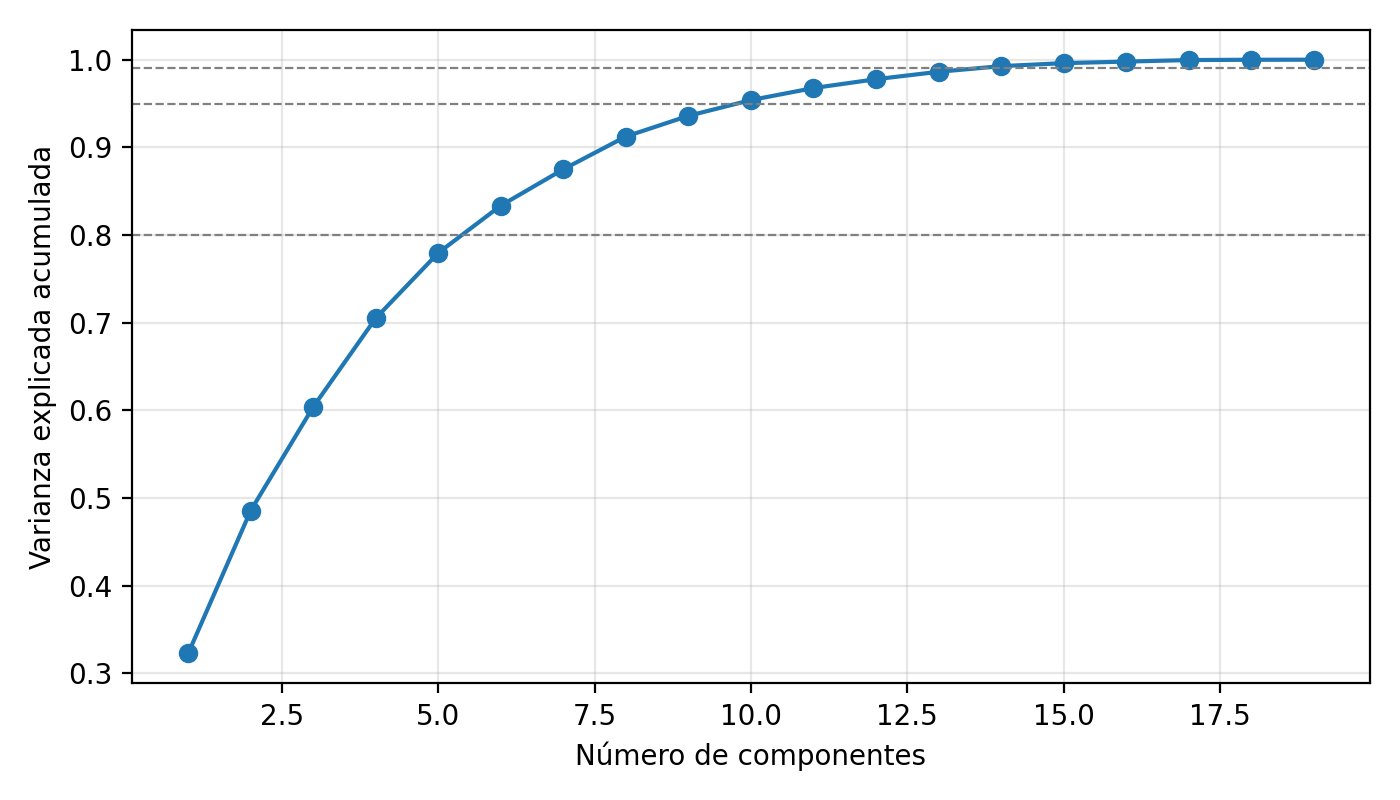
\includegraphics[width=0.9\columnwidth]{figures/pca_varianza.png}
  \caption{Varianza explicada acumulada por PCA en el conjunto de entrenamiento. Las líneas
  discontinuas marcan el 80\,\%, 95\,\% y 99\,\%.}
  \label{fig:pcavar}
\end{figure}

\begin{table*}[t]
\centering
\caption{Resultados con PCA (MCC, media $\pm$ 2 desviaciones estándar). La fila de 19 dimensiones
corresponde al modelo sin reducción. FP y FN se cuentan en prueba. Entrenamiento y validación de SVM
usan el subconjunto de 31.383 muestras.}
\label{tab:pca}
\small
\begin{tabular}{llcccccrr}
\toprule
\textbf{Modelo} & \textbf{Comp.} & \textbf{Reducción} & \textbf{MCC entren.} & \textbf{MCC valid.} &
\textbf{MCC prueba} & \textbf{Hiperparámetros} & \textbf{FP} & \textbf{FN} \\
\midrule
MLP & 19 & 0\,\% & 0,9959 $\pm$ 0,0006 & 0,9956 $\pm$ 0,0014 & 0,9960 $\pm$ 0,0008 & (128, 64, 32), $\alpha=10^{-4}$ & 2 & 91 \\
    & 14 & 26,3\,\% & 0,9960 $\pm$ 0,0002 & 0,9957 $\pm$ 0,0012 & 0,9958 $\pm$ 0,0009 & (128, 64, 32), $\alpha=10^{-4}$ & 17 & 79 \\
    & 10 & 47,4\,\% & 0,9924 $\pm$ 0,0021 & 0,9916 $\pm$ 0,0027 & 0,9901 $\pm$ 0,0013 & (64, 32), $\alpha=10^{-4}$ & 70 & 157 \\
    & 6 & 68,4\,\% & 0,9730 $\pm$ 0,0025 & 0,9718 $\pm$ 0,0025 & 0,9738 $\pm$ 0,0021 & (128, 64, 32), $\alpha=10^{-4}$ & 239 & 365 \\
\midrule
SVM & 19 & 0\,\% & 0,9957 $\pm$ 0,0010 & 0,9949 $\pm$ 0,0041 & 0,9961 $\pm$ 0,0008 & $C=100$, $\gamma=\texttt{scale}$ & 6 & 85 \\
    & 14 & 26,3\,\% & 0,9951 $\pm$ 0,0025 & 0,9932 $\pm$ 0,0016 & 0,9943 $\pm$ 0,0010 & $C=100$, $\gamma=\texttt{scale}$ & 22 & 110 \\
    & 10 & 47,4\,\% & 0,9841 $\pm$ 0,0019 & 0,9760 $\pm$ 0,0084 & 0,9810 $\pm$ 0,0018 & $C=100$, $\gamma=0{,}1$ & 126 & 313 \\
    & 6 & 68,4\,\% & 0,9738 $\pm$ 0,0077 & 0,9483 $\pm$ 0,0100 & 0,9539 $\pm$ 0,0028 & $C=100$, $\gamma=1$ & 350 & 712 \\
\bottomrule
\end{tabular}
\end{table*}

La Tabla~\ref{tab:pca} muestra que con 14 componentes MLP iguala al modelo sin reducción (MCC de
validación 0,9957 frente a 0,9956) y SVM queda apenas por debajo (0,9932 frente a 0,9949, con
intervalos que se solapan). Con el criterio del 95\,\%, 10 componentes, la pérdida ya es apreciable:
MLP baja a 0,9916 y SVM a 0,9760, y los errores de prueba se multiplican por más de dos. Con 6
componentes la caída es mayor. Esto indica que los últimos componentes, aunque explican poca
varianza, contienen información útil para separar las clases, porque PCA ordena los componentes por
varianza y no por su relación con la etiqueta. En SVM con 6 y 10 componentes, la brecha entre
entrenamiento y validación es mayor que en MLP, y el $\gamma$ elegido pasa de \texttt{scale} a
0,1 y 1.

\textbf{UMAP.} A diferencia de PCA, UMAP no ofrece una medida equivalente a la varianza explicada,
así que el número de componentes se elige de forma empírica comparando 2, 5 y 10 dimensiones; 10 es
la dimensión que retiene el 95\,\% de la varianza en PCA. Se usan los valores por defecto
$n_{\text{neighbors}}=15$ y $d_{\min}=0{,}1$. Por su costo, en cada pliegue UMAP aprende la proyección
con una muestra aleatoria de 20.000 URLs del entrenamiento y la aplica a las demás; luego sus
coordenadas se estandarizan, porque no tienen una escala definida.

\begin{table*}[t]
\centering
\caption{Resultados con UMAP (MCC, media $\pm$ 2 desviaciones estándar). La fila de 19 dimensiones
corresponde al modelo sin reducción. FP y FN se cuentan en prueba. Entrenamiento y validación de SVM
usan el subconjunto de 31.383 muestras.}
\label{tab:umap}
\small
\begin{tabular}{llcccccrr}
\toprule
\textbf{Modelo} & \textbf{Dim.} & \textbf{Reducción} & \textbf{MCC entren.} & \textbf{MCC valid.} &
\textbf{MCC prueba} & \textbf{Hiperparámetros} & \textbf{FP} & \textbf{FN} \\
\midrule
MLP & 19 & 0\,\% & 0,9959 $\pm$ 0,0006 & 0,9956 $\pm$ 0,0014 & 0,9960 $\pm$ 0,0008 & (128, 64, 32), $\alpha=10^{-4}$ & 2 & 91 \\
    & 10 & 47,4\,\% & 0,8204 $\pm$ 0,0069 & 0,8196 $\pm$ 0,0075 & 0,8313 $\pm$ 0,0050 & (128, 64, 32), $\alpha=10^{-4}$ & 727 & 3.212 \\
    & 5 & 73,7\,\% & 0,8116 $\pm$ 0,0090 & 0,8110 $\pm$ 0,0152 & 0,8290 $\pm$ 0,0050 & (128, 64, 32), $\alpha=10^{-4}$ & 715 & 3.280 \\
    & 2 & 89,5\,\% & 0,7759 $\pm$ 0,0235 & 0,7755 $\pm$ 0,0278 & 0,7890 $\pm$ 0,0055 & (128, 64, 32), $\alpha=10^{-4}$ & 895 & 4.043 \\
\midrule
SVM & 19 & 0\,\% & 0,9957 $\pm$ 0,0010 & 0,9949 $\pm$ 0,0041 & 0,9961 $\pm$ 0,0008 & $C=100$, $\gamma=\texttt{scale}$ & 6 & 85 \\
    & 10 & 47,4\,\% & 0,8461 $\pm$ 0,0062 & 0,8312 $\pm$ 0,0166 & 0,8420 $\pm$ 0,0049 & $C=100$, $\gamma=1$ & 722 & 2.959 \\
    & 5 & 73,7\,\% & 0,8321 $\pm$ 0,0061 & 0,8226 $\pm$ 0,0157 & 0,8327 $\pm$ 0,0050 & $C=100$, $\gamma=1$ & 835 & 3.056 \\
    & 2 & 89,5\,\% & 0,6866 $\pm$ 0,0715 & 0,6816 $\pm$ 0,0730 & 0,6714 $\pm$ 0,0068 & $C=100$, $\gamma=1$ & 2.252 & 5.310 \\
\bottomrule
\end{tabular}
\end{table*}

La Tabla~\ref{tab:umap} muestra que UMAP pierde buena parte de la información: el mejor resultado,
SVM con 10 dimensiones, alcanza MCC de prueba 0,8420, muy por debajo de 0,9961. Pasar de 5 a 10
dimensiones apenas mejora, y con 2 la caída es mayor. Los errores son sobre todo \textit{phishing} no
detectado (entre 2.959 y 5.310 falsos negativos). La Fig.~\ref{fig:umap} explica este comportamiento:
en dos dimensiones, muchas URLs de ambas clases quedan en las mismas regiones, porque UMAP conserva
la vecindad local en el espacio de entrada sin usar la etiqueta. En SVM, $\gamma=1$ es el extremo de
la malla; un valor mayor podría mejorar algo, pero es poco probable que cierre una diferencia de 0,15
en MCC. Otra limitación es que la proyección se aprende con 20.000 de las 188.296 URLs de
entrenamiento.

\begin{figure}[t]
  \centering
  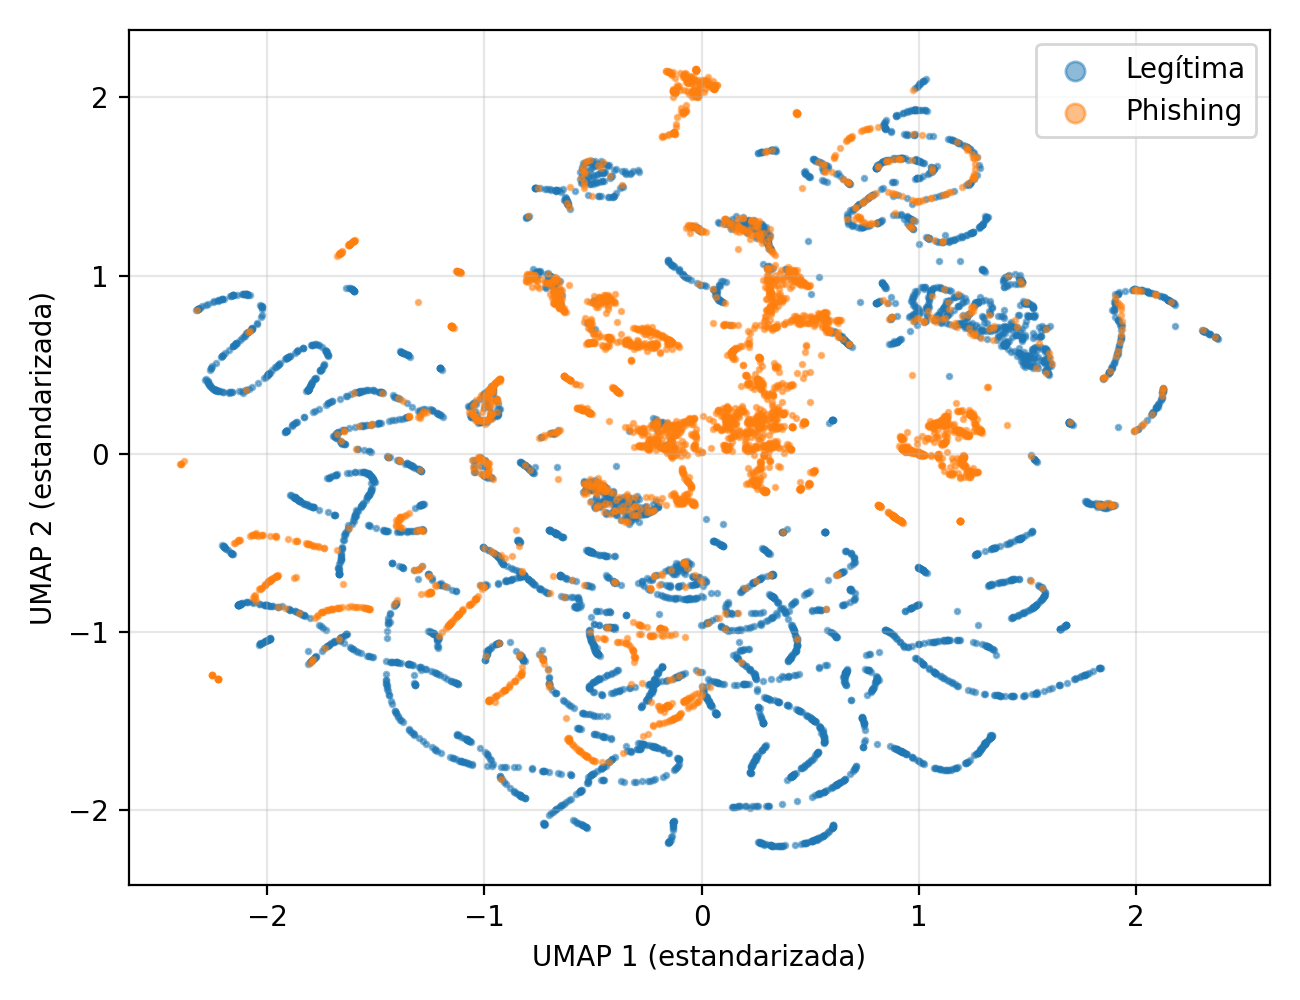
\includegraphics[width=0.9\columnwidth]{figures/umap_2d.png}
  \caption{Proyección UMAP en dos dimensiones de 8.000 URLs de prueba elegidas al azar, con la
  proyección aprendida en entrenamiento.}
  \label{fig:umap}
\end{figure}

\begin{figure}[t]
  \centering
  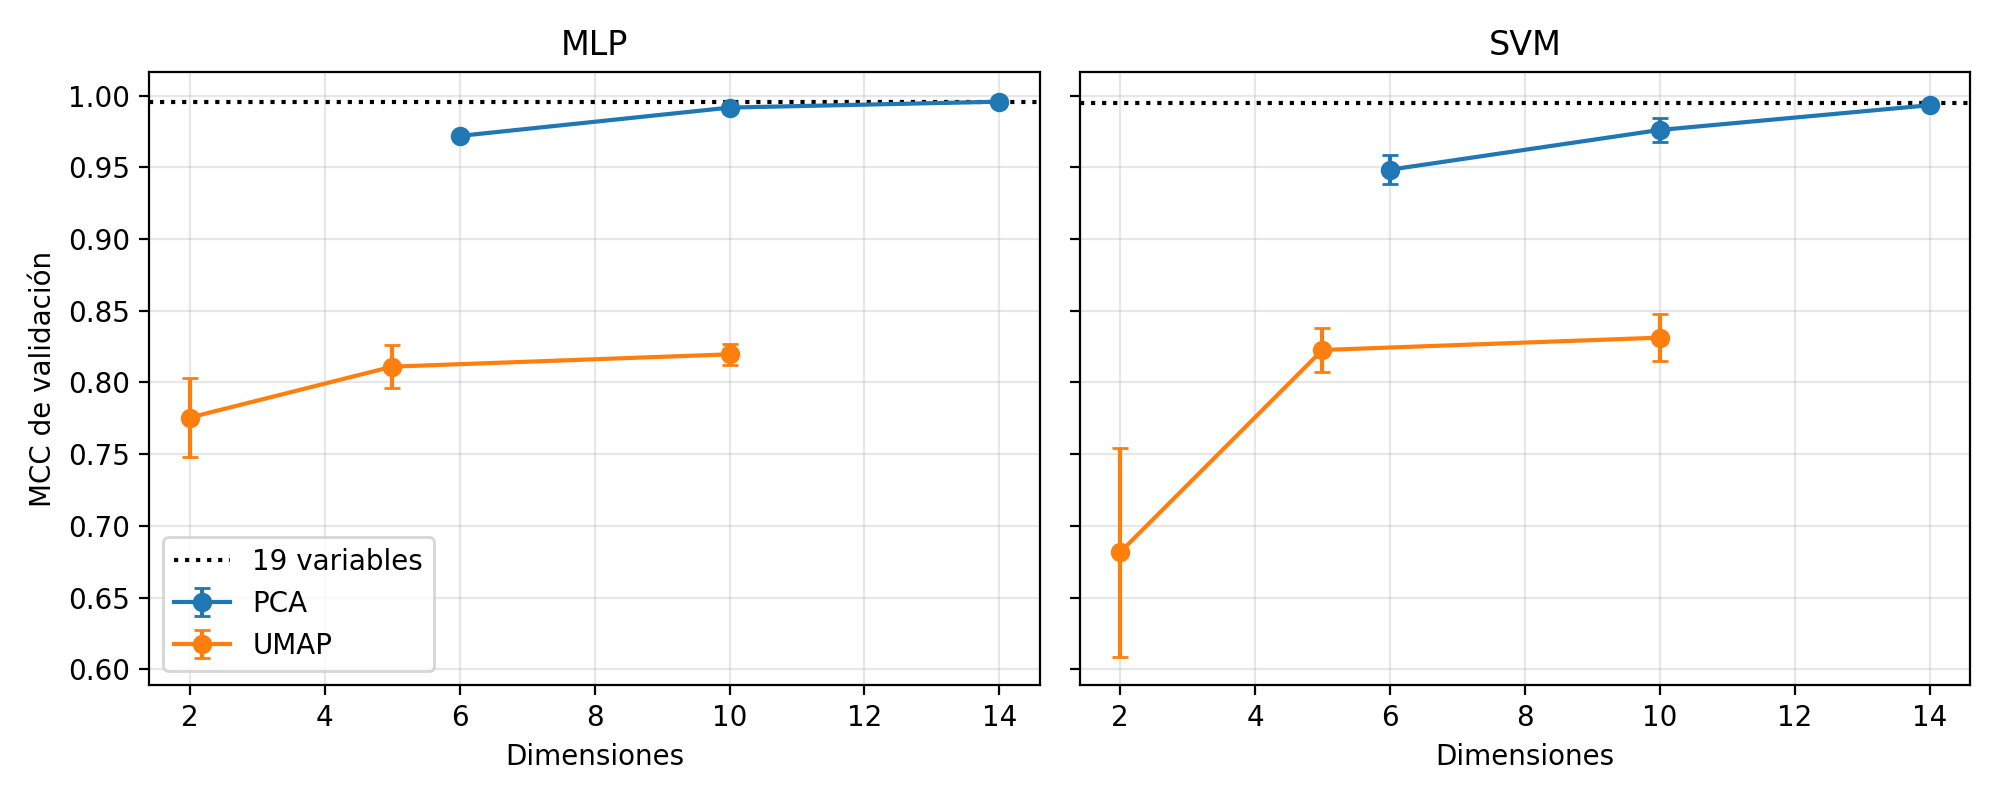
\includegraphics[width=\columnwidth]{figures/reduccion_comparacion.png}
  \caption{MCC de validación (media $\pm$ 2 desviaciones estándar) según el número de dimensiones
  con PCA y UMAP. La línea punteada es el resultado con las 19 variables.}
  \label{fig:reduccion}
\end{figure}

\subsection{Discusión}

La Fig.~\ref{fig:reduccion} resume la comparación con la Sección~\ref{sec:modelos}. La selección de
variables es la mejor opción: reduce el 52,6\,\% de las variables sin pérdida apreciable de MCC y
conserva variables interpretables, que además no hay que transformar antes de clasificar. PCA
mantiene el desempeño con 14 componentes (26,3\,\% de reducción), pero cada componente combina las
19 variables originales, así que no evita calcularlas. UMAP no es adecuado para este problema: incluso
con 10 dimensiones pierde más de 0,15 en MCC, y su ajuste es más costoso que el de PCA. En los tres casos, MLP
tolera mejor la reducción que SVM, con la excepción de UMAP con 5 y 10 dimensiones, donde SVM queda
levemente por encima.

%=============================================================================
\section{Discusión y conclusiones}
\label{sec:conclusiones}
%=============================================================================
\textbf{Comparación con el estado del arte.} En el escenario Completo, los cinco modelos alcanzan MCC
entre 0,9988 y 1,0000 en prueba, lo que coincide con las exactitudes superiores al 99\,\% de
\cite{prasad2024} y \cite{bao2026}. Sin embargo, en ese escenario también la regresión logística
llega a 0,9998, de modo que esas cifras reflejan sobre todo variables casi deterministas creadas
junto con el conjunto, como \texttt{URLSimilarityIndex} e \texttt{IsHTTPS}, y no la dificultad real
del problema. Al retirarlas, la regresión logística baja a 0,9090 y solo Random Forest, MLP y
SVM superan 0,99. Nuestro resultado en Solo URL es coherente con \cite{yulianti2026}, que también
excluye las variables con fuga y obtiene F1 de 0,9965 con 20 variables de la URL; MLP alcanza F1 de
validación 0,9975 con 19. Ambos trabajos coinciden además en que basta un subconjunto pequeño de
variables: \cite{yulianti2026} usa 5 elegidas con LASSO y aquí se conservan 9 sin pérdida
apreciable. Los trabajos de la Tabla~\ref{tab:sota} usan particiones estratificadas sin agrupar por
dominio; aquí, en cambio, la partición impide que URLs del mismo sitio aparezcan en entrenamiento y
prueba. El desempeño menor de \cite{gobinath2026}, 95\,\%
de exactitud, se obtiene combinando PhiUSIIL con otros dos conjuntos, lo que sugiere que el problema
es más difícil cuando las URLs provienen de fuentes distintas.

\textbf{Conclusiones.}
\begin{itemize}
  \item Con solo las 19 variables de la URL, MLP (MCC de prueba 0,9960 $\pm$ 0,0008) y SVM con
        \textit{kernel} RBF (0,9961 $\pm$ 0,0008) son los mejores modelos; sus intervalos se
        solapan y no muestran señales de sobreajuste. Los modelos lineales se quedan cerca de
        0,91, por lo que la frontera entre clases no es lineal.
  \item El error dominante es el \textit{phishing} no detectado: MLP comete 91 falsos negativos y
        2 falsos positivos en 47.074 URLs de prueba.
  \item La selección de variables reduce el espacio de 19 a 9 variables (52,6\,\%) sin pérdida
        apreciable de MCC. PCA requiere 14 componentes para conservar el desempeño y UMAP pierde
        más de 0,15 en MCC, de modo que la selección es la reducción más conveniente.
  \item Los resultados casi perfectos sobre PhiUSIIL deben interpretarse con cautela, porque
        dependen de cómo se construyó el conjunto.
\end{itemize}

\textbf{Limitaciones y trabajo futuro.} Incluso en Solo URL, las URLs legítimas conservan una
estructura propia del conjunto: todas empiezan por \texttt{www} y ninguna tiene ruta, de modo que
parte del desempeño puede deberse a esa diferencia y no a patrones propios del \textit{phishing}.
Además, SVM se entrenó con un subconjunto de 31.383 muestras y UMAP aprendió la proyección con
20.000. Como trabajo futuro se propone evaluar los modelos con URLs legítimas que incluyan rutas y
parámetros, y con conjuntos de datos de otras fuentes, para medir su capacidad de generalizar a
sitios reales.

%=============================================================================
\begin{thebibliography}{1}
\bibitem{prasad2024}
A. Prasad and S. Chandra, ``PhiUSIIL: A diverse security profile empowered phishing URL
detection framework based on similarity index and incremental learning,''
\emph{Computers \& Security}, vol. 136, art. no. 103545, 2024,
doi: 10.1016/j.cose.2023.103545.

\bibitem{gobinath2026}
R. Gobinath and S. Manikandan, ``Deep learning-based phishing classification framework for
accurate detection using optimized URL intelligence,'' \emph{Scientific Reports}, vol. 16,
art. 15794, 2026, doi: 10.1038/s41598-026-46481-2.

\bibitem{bao2026}
T. M. Bao, K. Shashvat, N. G. Nhu, and D.-N. Le, ``A comparative analysis of machine learning
algorithms for spam and phishing URL classification,'' \emph{Computers, Materials \& Continua},
vol. 87, no. 2, art. no. 35, 2026, doi: 10.32604/cmc.2025.075161.

\bibitem{yulianti2026}
F. Yulianti and J. Forenziana, ``A comparative analysis of feature selection methods for
machine learning-based phishing URL detection,'' \emph{Formosa Journal of Computer and
Information Science}, vol. 5, no. 2, pp. 243--258, 2026, doi: 10.55927/fjcis.v5i2.16783.
\end{thebibliography}

\end{document}
